\documentclass[a4paper,oneside,bibtotoc,smallheadings,pointlessnumbers,
halfparskip,DIV15]{scrartcl}
% kate: remove-trailing-space on; replace-trailing-space-save on; indent-width 2; indent-mode normal; space-indent on;
% tocleft,
\usepackage[pdftex]{graphicx}
\usepackage[ngerman]{babel}
\usepackage[utf8]{inputenc}
\usepackage{../../assets/uniinput}
\usepackage[T1]{fontenc}
\usepackage{amssymb,amsmath}
\usepackage{booktabs}
\usepackage{enumerate}
\usepackage{subfig}
% \usepackage{siunitx}
% \sisetup{
%   seperr         = true,
%   trapambigerr   = true,
%   openerr        = (,
%   closeerr       = ),
%   expproduct     = cdot,
%   padnumber      = both,
%   stickyper      = true,
%   per            = reciprocal,
%   trapambigfrac  = true,
%   repeatunits    = false,
%   openfrac       = (,
%   closefrac      = ),
%   prefixsymbolic = true,
%   prefixproduct  = cdot,
%   decimalsymbol  = comma,
%   tabnumalign    = left,
%   tabtextalign   = left
% }
\usepackage{color}
\definecolor{grey}{rgb}{.4,.4,.4}
\definecolor{darkgreen}{rgb}{0,.35,0}
\definecolor{ltgray}{gray}{0.95}
% \definecolor{darkblue}{rgb}{0,0,.6}
% \definecolor{darkred}{rgb}{.6,0,0}
% \definecolor{red}{rgb}{.98,0,0}
\usepackage{listings}
\lstdefinelanguage{Maxima}{
  keywords={addrow,addcol,zeromatrix,ident,augcoefmatrix,ratsubst,diff,ev,tex,%
    with_stdout,nouns,express,depends,load,submatrix,div,grad,curl,%
    rootscontract,solve,part,assume,sqrt,integrate,abs,inf,exp,float,log},
  sensitive=true,
  comment=[n][\itshape]{/*}{*/}
}
\lstdefinelanguage{C++}{
%   commentstyle=\itshape\color{darkgreen},
%   commentstyle=\color{darkgreen},
%   keywordstyle=\bfseries, %\color{darkblue},
%   stringstyle=\color{darkred},
%   basicstyle=\ttfamily\scriptsize,
  morekeywords={TH1F,TLorentzVector,TVector3,vector,TFile,TFitResultPtr,TF1,\
                TGraph,TH1,TObject,TCanvas,string,Double_t,TGraphErrors},
  basicstyle=\scriptsize,
  numbers=left,
  numberstyle=\tiny,%\color{gray},
  stepnumber=1,
  tabsize=4,
  showspaces=false,
  showstringspaces=false,
  breaklines=true,
  frame=lrtb,
  captionpos=b,
  extendedchars=true,
  inputencoding=utf8,
%   backgroundcolor=\color{ltgray}
}
% \usepackage{courier}
\lstset{language=Matlab,
%     keywords={break,case,catch,continue,else,elseif,end,for,function,global,if,otherwise,persistent,return,switch,try,while},
%     basicstyle=\ttfamily\small,%\scriptsize,
  basicstyle=\scriptsize,
  keywordstyle=\bfseries,
  commentstyle=\itshape\color{blue},
  stringstyle=\itshape,
  identifierstyle=\ttfamily,
  numbers=left,
  numberstyle=\tiny,
  stepnumber=1,
  tabsize=2,
  showspaces=false,
  showstringspaces=false,
  breaklines=true,
  frame=single,
  columns=fixed,
  captionpos=b,
  extendedchars=\true,
  inputencoding=utf8,
  backgroundcolor=\color{ltgray},
  postbreak = \raisebox{0ex}[0ex][0ex]{\ensuremath{\hookrightarrow}}
%   linewidth=0.9\textwidth
}
\usepackage[pdftex]{hyperref}
\hypersetup{
%   colorlinks  = true,
%   urlcolor    = darkblue,
  pdftitle    = {Protokoll zum CPII-Übungsblatt 4},
  pdfsubject  = {Protokoll Computational Physics}
  pdfauthor   = {robert.riemann@physik.hu-berlin.de,thomas.murach@physik.hu-berlin.de},
%   pdfkeywords = {Computational Physics,CP,II,2010,Jacobi-Methode,Diagonalisierung,Eigenwerte, Eigenvektoren,eig,octave,matlab}
%   pdfcreator  = {pdftex},
%   pdfproducer = {pdftex}
}

\newcommand{\dd}[1]{\mathrm{d}#1\,} % declare dx operator, usage: \dd{x} for dx
\newcommand{\lref}[1]{Listing (\ref{lst:#1})} % refer to a listing, usage: \lref{label} for Listing (...)
\newcommand{\fref}[1]{Abb. (\ref{fig:#1})} % refer to a figure, usage: \lref{label} for Abb. (...)
\newcommand{\tref}[1]{Tab. (\ref{tab:#1})} % refer to a table, usage: \lref{label} for Tab. (...)
\newcommand{\eref}[1]{Gl. (\ref{eqn:#1})} % refer to a equation, usage: \lref{label} for Tab. (...)

\begin{document}
% % % % % % % % % % % % % % % % % % % % % % % %
\title{{\centering \rule{15cm}{0.001cm}\\
\Large{\textsc{Institut für Physik der
Humboldt-Universität zu Berlin}}}\\ \centering \rule{15cm}{0.001cm}\\
\vspace{15mm} \centering

\includegraphics[scale=0.9]{../../assets/siegel}\\
\vspace{18mm}
{\bf{\huge{Computational Physics II}}}\\
\vspace{12mm}
Übungsblatt 4\\
\vspace{15mm}
% Compton-Effekt\\
% \vspace{14mm} {\small{\textbf{Betreuer: M. zur Nedden}}}\\}
}
\author{Robert Riemann; Matr.Nr.: 521085\\
Thomas Murach; Matr.Nr.: 517771\vspace{18mm}}
% \vspace{8mm}
% \date{15. Juni 2008}
% % % % % % % % % % % % % % % % % % % % % % % %
% \onecolumn
\maketitle
% \twocolumn

\newpage
% \tableofcontents
% \listoffigures
% \listoftables
\section*{Aufgabe 5.1}
Im Folgenden wurde mittels der Fourier-Analyse eine Möglichkeit der Bildkomprimierung
getestet. Das in Matlab als $(m\times n)$-Matrix importierte Bild ohne Veränderungen ist
in \fref{orig} abgebildet. Die Matrix enthält die Graustufenwerte als Fließkommazahlen
(\texttt{double}).

\begin{figure}[htb]
\centering
  
\includegraphics[width=0.7\textwidth,keepaspectratio]{../tmp/original}
  \caption{Orginales Bild ohne Komprimierung}
  \label{fig:orig}
\end{figure}

\section*{Aufgabe 5.1a)}

Zunächst wurde eine Funktion \lref{cut_rect} geschrieben, die den Rand des Graustufen-Bildes
schwärzt, die Pixel also auf 0 setzt. Die Breite wird hierbei in Abhängigkeit
des Kompressionsparameters $ρ \in ]0,1]$ so eingestellt, dass $hb\cdot ρ^2$
nicht-triviale Pixel verbleiben, wobei $h$ die Höhe und $b$ die Breite des
Bildes in Pixeln ist.

Wird die Funktion aus \lref{cut_rect} unter Verwendung von $ρ^2 = 0.4$ auf das
Bild in \fref{orig} angewendet, so erhält man die in \fref{1a} gezeigte Abbildung.
\lstinputlisting[firstline=1,lastline=8,firstnumber=1,label=lst:fft-test,caption={blatt5.m}]{../code/blatt5.m}
\lstinputlisting[firstline=1,lastline=10,firstnumber=1,label=lst:cut_rect,caption={cut\_rect.m}]{../code/cut_rect.m}

\begin{figure}[htb]
\centering
  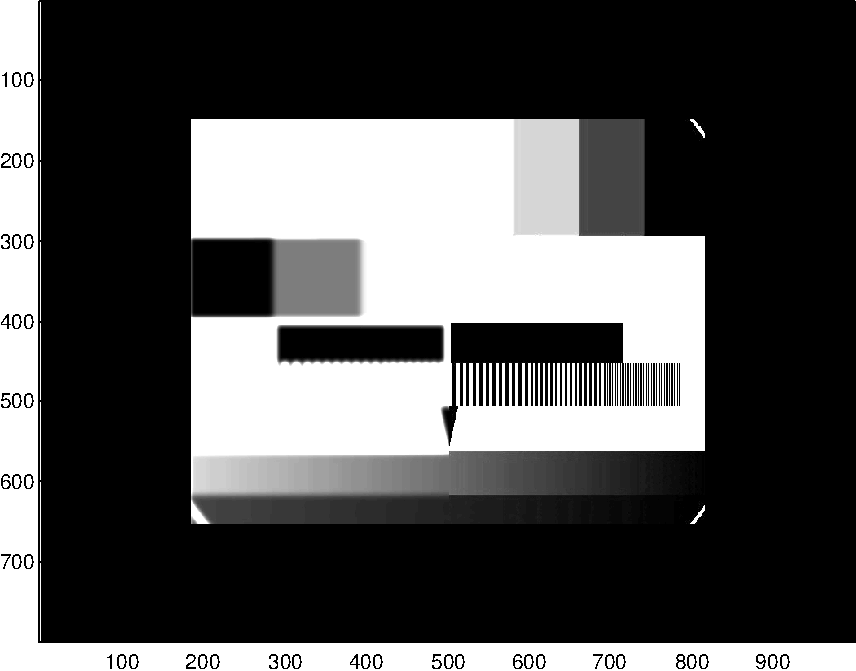
\includegraphics[width=0.7\textwidth,keepaspectratio]{../tmp/eins_a-crop.pdf}
  \caption{Bild mit Rand bei $ρ^2 = 0.4$}
  \label{fig:1a}
\end{figure}

Wie man erkennen kann, wurde abgesehen von der gewünschten Rahmen-Erzeugung
auch der innere Bereich des Bildes verändert, was allerdings nicht ein Effekt der
Beschneidung ist, sondern vermutlich auf die begrenzte Auflösung der Farbskala 
zurückzuführen ist. Daher sind beispielsweise die in der Bildmitte befindlichen
hellgrauen Blöcke im transformierten Bild nicht mehr zu finden. 

\section*{Aufgabe 5.1b)}
Für die folgenden Aufgaben wurden die in Matlab zur Verfügung stehenden 
Fast-Fourier-Transformationsfunktionen \texttt{fft, ifft, fft2, ifft2} benötigt.
Zunächst wurde getestet, wie diese funktionieren, indem mit einfachen Vektoren und
Matrizen eine Hin- und eine Rücktransformation durchgeführt wurde, wie in 
\lref{fft-test} gezeigt.
\lstinputlisting[firstline=10,lastline=23,firstnumber=10,label=lst:fft-test,caption={blatt5.m}]{../code/blatt5.m}

Der zugehörige Output ist in \lref{fft-test-output} gezeigt.
\begin{lstlisting}[caption=Output des Beispielaufrufs,label=lst:fft-test-output]
a =

    0.0759
    0.0540
    0.5308
    0.7792
    0.9340


a_fft =

   2.3738          
  -0.6786 + 0.9830i
  -0.3186 + 0.2811i
  -0.3186 - 0.2811i
  -0.6786 - 0.9830i


a_2 =

    0.0759
    0.0540
    0.5308
    0.7792
    0.9340


a_fftshift =

    0.7792
    0.9340
    0.0759
    0.0540
    0.5308


a_ifftshift =

    0.0759
    0.0540
    0.5308
    0.7792
    0.9340


A =

    0.1299    0.1622    0.6020    0.4505    0.8258
    0.5688    0.7943    0.2630    0.0838    0.5383
    0.4694    0.3112    0.6541    0.2290    0.9961
    0.0119    0.5285    0.6892    0.9133    0.0782
    0.3371    0.1656    0.7482    0.1524    0.4427


A_fft =

  11.1456            -0.8578 + 0.2117i  -0.9221 + 1.6125i  -0.9221 - 1.6125i  -0.8578 - 0.2117i
  -0.5132 - 0.6404i   0.6573 - 1.2749i  -0.1080 + 1.1941i  -0.2687 + 0.1951i   0.3350 - 1.9203i
   0.3664 + 0.1807i  -1.9259 + 1.5904i  -1.8499 + 0.0229i   1.4279 - 0.0361i  -0.2900 - 0.2633i
   0.3664 - 0.1807i  -0.2900 + 0.2633i   1.4279 + 0.0361i  -1.8499 - 0.0229i  -1.9259 - 1.5904i
  -0.5132 + 0.6404i   0.3350 + 1.9203i  -0.2687 - 0.1951i  -0.1080 - 1.1941i   0.6573 + 1.2749i


A_2 =

    0.1299    0.1622    0.6020    0.4505    0.8258
    0.5688    0.7943    0.2630    0.0838    0.5383
    0.4694    0.3112    0.6541    0.2290    0.9961
    0.0119    0.5285    0.6892    0.9133    0.0782
    0.3371    0.1656    0.7482    0.1524    0.4427


A_fftshift =

    0.9133    0.0782    0.0119    0.5285    0.6892
    0.1524    0.4427    0.3371    0.1656    0.7482
    0.4505    0.8258    0.1299    0.1622    0.6020
    0.0838    0.5383    0.5688    0.7943    0.2630
    0.2290    0.9961    0.4694    0.3112    0.6541


A_ifftshift =

    0.1299    0.1622    0.6020    0.4505    0.8258
    0.5688    0.7943    0.2630    0.0838    0.5383
    0.4694    0.3112    0.6541    0.2290    0.9961
    0.0119    0.5285    0.6892    0.9133    0.0782
    0.3371    0.1656    0.7482    0.1524    0.4427
\end{lstlisting}

Wie man erkennen kann, sind die Vektoren und Matrizen nach zwei Transformationen
gleich den hineingesteckten Objekten, sodass die grundlegende Funktionalität als
gegeben angenommen werden kann.

Weiterhin wurden die Funktionen \texttt{fftshift} und \texttt{ifftshift}
untersucht (siehe \lref{fft-test}). Diese führen zunächst eine Hin- bzw. Rücktransformation
durch und verschieben die $k$-Werte in der Art, dass pro Zeile und Spalte die 
zu $k=0$ gehörenden Werte in die Mitte gelangen. Dies entspricht einer Symmetrisierung.
Die Funktion \texttt{ifftshift} macht diese Symmetrisierung wieder rückgängig, um
die ursprüngliche Matrix wiederzubekommen.

Die beiden Funktionen \textcolor{red}{unterscheiden} sich aufgrund der Nichtlinearität der Abhängigkeit
von $x$ und $k$. (oder: octave- help fftshift -> laenge spielt eine rolle)


\section*{Aufgabe 5.1c)}
Zur Komprimierung des Bildes aus \fref{orig} wird eine 2D-Fourier-Transformation
in den $k$-Raum durchgeführt. Im Anschluss wird das Bild symmetrisiert, die Bildinformation
auf $hb\cdot ρ^2$ durch das Abschneiden des Randes reduziert, die Symmetrisierung wieder
rückgängig gemacht und zuletzt wird das Bild wieder durch die inverse Fourier-Trafo in den
$x$-Raum überführt.

Das Ergebnis für $ρ=0.5$ ist in \fref{1c5} und für $ρ=0.1$ ist in \fref{1c1} dargestellt.

\begin{figure}[htb]
\centering
  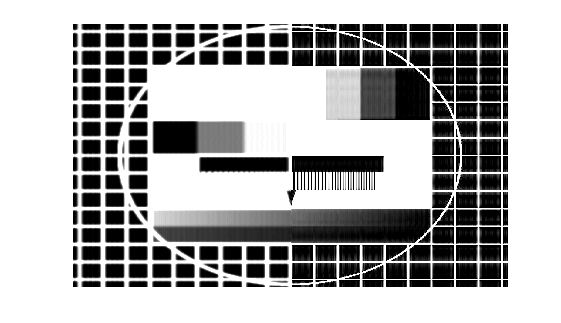
\includegraphics[width=0.7\textwidth,keepaspectratio]{../tmp/eins_c_0_5}
  \caption{komprimiertes Bild mit rechteckigem Rand im $k$-Raum, $ρ=0.5$}
  \label{fig:1c5}
  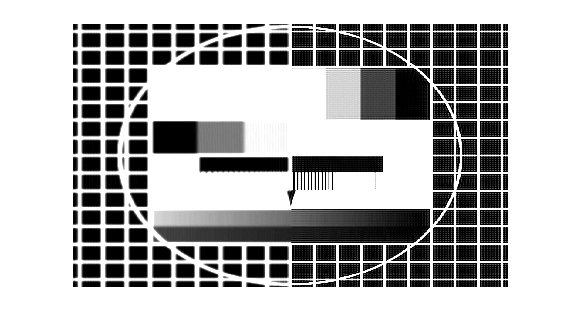
\includegraphics[width=0.7\textwidth,keepaspectratio]{../tmp/eins_c_0_1}
  \caption{komprimiertes Bild mit rechteckigem Rand im $k$-Raum, $ρ=0.1$}
  \label{fig:1c1}
\end{figure}

\section*{Aufgabe 5.1d)}

In Aufgabe d) wurde equivalent zur Verfahrensweise in c) vorgegangen.
Jedoch wurde im transformierten Raum nicht ein rechteckiger Rand abgeschnitten,
sondern ein Kreisförmiger, siehe \lref{cut_round}. Hierbei wurde darauf geachtet, dass die verbleibende
Bildinformation nach wie vor $hb\cdot ρ^2$ ist.

\lstinputlisting[firstline=1,lastline=15,firstnumber=1,label=lst:cut_round,caption={cut\_round.m}]{../code/cut_round.m}

\begin{figure}[htb]
\centering
  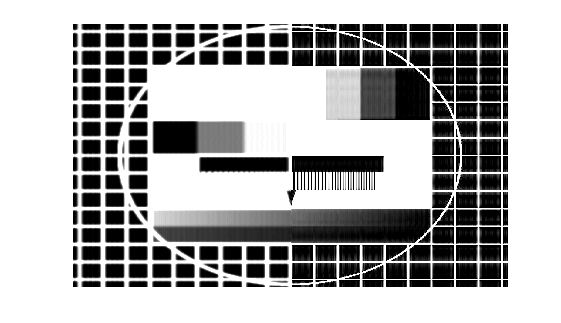
\includegraphics[width=0.7\textwidth,keepaspectratio]{../tmp/eins_c_0_5}
  \caption{komprimiertes Bild mit kreisförmigen Rand im $k$-Raum, $ρ=0.5$}
  \label{fig:1d5}
\end{figure}

Im Vergleich zu \fref{1a} kann man erkennen, dass, abgesehen davon, dass kein
Rahmen zum Bild hinzugefügt wurde, das Bild selbst verändert wurde. 

\section*{Aufgabe 5.1d)}
Hier wurde der Schnitt auf den Betrag von $k$ angewandt und nicht wie bisher
auf die einzelnen Komponenten. Der aufrufende Quelltext ist in \lref{k_kreis} und 
die aufgerufene Funktion \texttt{cut\_round} dargestellt.

\lstinputlisting[firstline=32,firstnumber=32,label=lst:k_kreis,caption={blatt5.m}]{../code/blatt5.m}
\lstinputlisting[label=lst:cut_round,caption={cut\_round.m}]{../code/cut_round.m}

Die hierbei resultierenden Graphiken sind in \fref{kreis_0_1} (für $k = 0.1$) und
\fref{kreis_0_5} (für $k=0.5$) dargestellt.

\begin{figure}[htb]
\centering
  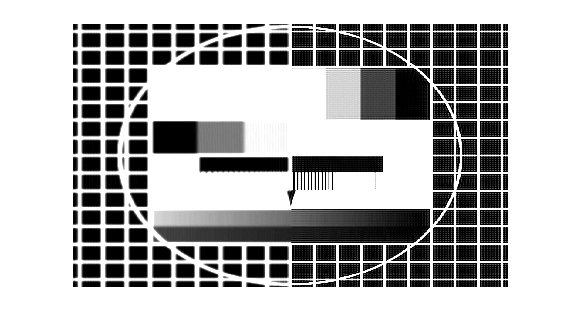
\includegraphics[width=0.7\textwidth,keepaspectratio]{../tmp/eins_c_0_1}
  \caption{komprimiertes Bild mit kreisförmigen Rand im $k$-Raum, $ρ=0.1$}
  \label{fig:1d1}
\end{figure}

Durch die Komprimierung, verändert sich das Bild. Das Ausmaß der Veränderung
hängt von der lokalen Struktur des Bildes ab. So kann man erkennen, dass
große einfarbige Flächen substrukturen aufweisen, also nicht sehr gut erhalten
bleiben. Dagegen bleiben periodische Muster, wie z.\,B. das Gitter, sehr gut
erhalten. Jedoch verschwimmen auch hier etwas Grenzen.

Farbverläufen erkennt man nach der Komprimierung deutlich die diskreten Stufen an.

Die Ergebnisse können folgendermaßen erklärt werden: Flächen entsprechen einem Plateau,
welches für eine gute Annäherung auch sehr hohe Frequenzen benötigt, welche wir jedoch
abgeschnitten haben. Daher erkennt man periodische Substrukturen.

Das Gitter selbst ist periodisch und weißt nur sehr kurze Plateaus (Peaks) auf, die auf Grund
der periodischen Natur der Fourier-Transformation im $k$-Raum auch ohne hohe Frequenzen
gut wiedergegeben werden können.

Wird eine höhere Kompression gewählt, so werden die Substrukturen deutlicher.

Die unterschiedlichen Werte für ϱ äußern sich hier in ein wenig anderen Artefakten. 
Die beiden hellgrauen Blöcke in der rechten Mitte der Bilder sind für $ϱ²=0.5$
annähernd homogen ausgefüllt, während für $ϱ²=0.1$ eine deutliche Strukturierung
zu erkennen ist. Im ursprünglichen Bild waren diese Bereiche homogen (oberer Block)
oder vertikal gestreift (unterer Block). Eine geringere Beschneidung im $k$-Raum
führt also zu einer tendenziell größeren Erhaltung der Informationen, was auch zu
erwarten war.

\section*{Aufgabe 5.1e)}
% \section*{3.1b)}

Zu zeigen ist der Zusammenhang, der zwischen der logistischen Abbildung mit $r = 4$
\begin{equation}
 M_L(x_n) = 4x_n(1-x_n) = x_{n+1}
 \label{eqn:ml}
\end{equation}
und der Dreiecksabbildung
\begin{equation}
 \label{eqn:md}
 M_D(x_n) = \left(1-2\left|\frac{1}{2}-x\right|\right) = x_{n+1}
\end{equation}
besteht.

Nun substituieren wir $x_n$ in \eref{ml} mit:
\begin{equation}
 x_n = \sin^2\left(\frac{\pi}{2}\alpha_n\right)
\end{equation}
Hierbei wird darauf geachtet, dass die Substitution selbst auch eine Abbildung
von $[0, 1]$ nach $[0, 1]$ darstellt. Man erhält:
\begin{eqnarray}
 M_L(x_n) = x_{n+1} &=& 4x_n(1-x_n) \\
 \sin^2\left(\frac{\pi}{2}\alpha_{n+1}\right) &=& 4\sin^2\left(\frac{\pi}{2}\alpha_n\right)\underbrace{\left(1-\sin^2\left[\frac{\pi}{2}\alpha_n\right]\right)}_{\cos^2\left(\frac{\pi}{2}\alpha_n\right)} \\
 &=& 4\left[ \sin\left(\frac{\pi}{2}\alpha_n\right)\cos\left(\frac{\pi}{2}\alpha_n\right)\right]^2 = 4 \left[ \frac{1}{2} \sin\left( 2 \frac{\pi}{2} \alpha_n \right) \right]^2 = \sin^2\left(\frac{\pi}{2}2\alpha_n\right) \\
 \rightarrow \alpha_{n+1} &=& \pm 2 \alpha_n
\end{eqnarray}

Wie aus der Vorlesung bekannt ist, hat die logistische Abbildung ebenfalls eine
Stretching-Wirkung mit Faktor 2. Das Vorzeichen hängt hierbei von $x$ ab und ist
für Werte $\in [0; 0.5]$ positiv.

Darauf folgt die Equivalenz des invarianten Maßes der Dreiecksabbildung $ρ_D = 1$
und der logistischen Abbildung in Abhängigkeit von $alpha$ $ρ_L(α)$:
\begin{equation}
 ρ_D = ρ_L(α) = 1 
\end{equation}
Es gilt weiterhin:
\begin{eqnarray}
 ρ_L(α)\dd{α} &=& ρ_L(x)\dd{x} \\
  \rightarrow ρ_L(x) &=& \underbrace{ρ_L(α)}_{=1} \frac{\dd{\alpha}}{\dd{x}} \\
 \frac{\dd{x}}{\dd{α}} &=&  π \sin\left(\frac{\pi}{2}\alpha\right)\cos\left(\frac{\pi}{2}\alpha\right) = π\sqrt{x(1-x)} \\
 \rightarrow ρ_L(x) &=& \frac{1}{\pi\sqrt{x(1-x)}}
\end{eqnarray}

Der Vergleich zwischen experimentellem und theoretischem Ergebnis ist in \fref{1b}
veranschaulicht. Die rote Line beschreibt den auf die experimentellen Daten
renormierten theroretischen Verlauf $ρ_L(x)$.
\begin{figure}[htb]
\centering
  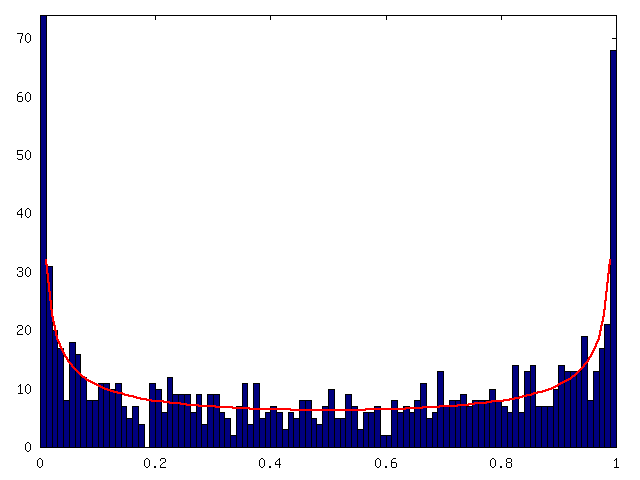
\includegraphics[width=1\columnwidth,keepaspectratio]{../logabb_r4.png}
  \caption{Vergleich zwischen Experiment und Theorie von $ρ_L(x)$}
  \label{fig:1b}
\end{figure}






\section*{Aufgabe 8.2}
In dieser Aufgabe sollte die Dichte in Abhängigkeit der Dichte für verschieden Gittergrößen
geplottet werden. Der Code dafür ist bereits in \lref{bond_perk} dargestellt. Die
resultierenden Kurven sind in \fref{dichte} dargestellt.

\begin{figure}[htb]
  \centering
  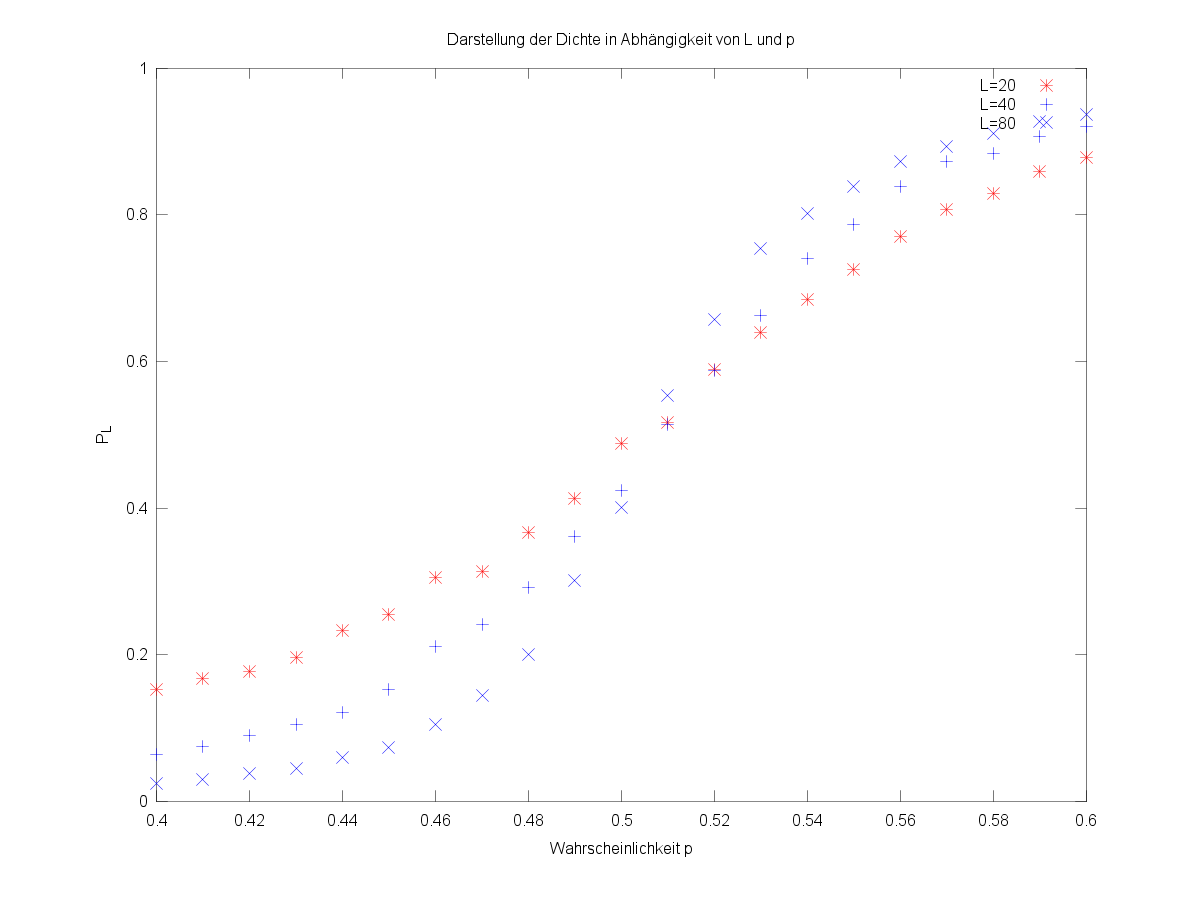
\includegraphics[width=0.8\columnwidth,keepaspectratio]{../tmp/zweitens.png}
  \caption{Dichte in Abhängigkeit von der Wahrscheinlichkeit und für verschiedene Gittergrößen}
  \label{fig:dichte}
\end{figure}

Man erwartet für $p<0.5$, dass die Dichte für sehr große Gitter gegen null geht 
und für größere Wahrscheinlichkeiten gegen 1. Dies kann hier nicht exakt erreicht werden,
da nur endliche Gitter verwendet wurden, aber die entsprechende Tendenz ist erkennbar.
Aufgrund der relativ langwierigen Programmausführung wurde sich auf drei Messwerte beschränkt.
% \input{auswertung}
% \input{ergebnis}
% \input{quellen}
% \input{anhang}

% \section{Beispiele}
% blabla
%
% Weitere Information sind der Versuchsbeschreibung im \cite{script} zu entnehmen.
%
% \lstinputlisting[firstline=2,firstnumber=1,label=lst:aufruf,caption={aufruf.m - Matlab Batchdatei}]{aufruf.m}
%
% \begin{eqnarray}
% 	g &=& \SI{9.8157(11)}{\metre\per\second\squared} \\
%         \left[ g \right] &=& \si{\metre\per\Square\second} % großschreibung!
% 	\label{eqn:asdf}
% \end{eqnarray}
%
% Dann kann man auf \eref{asdf} verweisen.


% \begin{figure}[htb]
% 	\centering
% 	\includegraphics[width=1\columnwidth,keepaspectratio]{Winkelabhaengigkeit2}
% 	\caption{Periodendauer in Abhängigkeit der Maximalauslenkung}
% 	\label{fig:Winkelabhaengigkeit}
% \end{figure}

% \begin{table}[htbp]
% \centering
% \setlength{\tabcolsep}{14pt}
% \begin{tabular*}{\columnwidth}{%
% S[tabformat=2.1]%
% S[tabformat=2.2]%
% S[tabformat=1.2]}
% \toprule
% {$R$ in \si{\ohm}} &
% {$U$ in \si{\volt}} &
% {$\frac{U}{U_{R=0}}$}\\
% \midrule
% \multicolumn{3}{c}{\textit{Eingangswiderstand $R_E$}}\\
% \midrule
% 0 & 16 & 1 \\
% 4.7e3 & 8 & 0.5 \\
% \midrule
% \multicolumn{3}{c}{\textit{Ausgangswiderstand $R_A$}}\\
% \midrule
% 0 & 1.8 & 1 \\
% 12 & 0.52 & 0.29 \\
% 27 & 1.2 & 0.67 \\
% 18 & 0.8 & 0.44 \\
% \bottomrule
% \end{tabular*}
% \label{tab:221messungexp_widerstaende}
% \caption{experimentelle Messung der Ein- und Ausgangswiderstände}
% \end{table}


% \newpage

% \onecolumn
% \appendix
% \begin{figure}
% 	\centering
% 	\includegraphics[width=0.98\textwidth,keepaspectratio]{Messprotokoll}
% 	\caption{Messprotokoll}
% 	\label{fig:protokoll}
% \end{figure}
%\colorbox{yellow}{} Farben verwenden
\end{document}
